%!TEX root = ../thesis.tex
%*******************************************************************************
%****************************** Third Chapter **********************************
%*******************************************************************************
\chapter{Neuromorphic Modelling}

\section[Introduction]{Introduction}

The brain is capable of performing a vast array of computations, with the fundamental units of the brain generally considered to be neurons and synapses. In the context of the nervous system, a synapse is defined as a structure that is capable of facilitating the transfer of an electrical or chemical signal from a presynaptic neuron to a postsynaptic neuron. \\

\noindent In the case of a chemical synapse, the occurrence of a spike in the presynaptic neuron will result in the stimulation of the release of a chemical substance known as a neurotransmitter. Subsequently, the neurotransmitter will migrate to bind with the receptors in the membrane of the postsynaptic neuron. \\

\noindent The effects of different neurotransmitters vary, exerting excitatory or inhibitory effects on the postsynaptic neurons. Many receptors contain different ion channels, which permit ions to flow between the inside and outside of the membrane, thereby generating an excitatory postsynaptic current (EPSC) or an inhibitory postsynaptic current (IPSC). \\

\noindent This chapter offers a concise overview of the pertinent biological details, along with the concepts and models from computational neuroscience that are employed or expanded upon in this study. These details provide invaluable preliminary information for accurately modelling the implementation of silicon oxide device-based neuromorphic hardware and bio-inspired computing.

\subsection[Neuroscience Primers]{Neuroscience Primers}

Computational neuroscience employs a computational methodology to elucidate the mechanisms underlying brain function. This entails not only identifying the computations performed by the brain but also understanding the interactions between brain elements, such as neurons and synapses, that facilitate these computations.\\

\noindent The field of computational neuroscience has traditionally adopted a bottom-up approach, commencing with the study of individual neurons and subsequently examining how these can be integrated into progressively larger networks, ultimately leading to the emergence of meaningful behaviour. In contrast, psychology and cognitive science have adopted a more top-down approach, commencing with the observation of animal behaviour and subsequently attempting to elucidate the brain mechanisms underlying these behaviours in terms of the higher-level functions of large brain areas. \\

\noindent This distinction has resulted in a historical focus on developing comprehensive mathematical models of individual neurons and small- to medium-sized networks in computational neuroscience. Recently, however, there has been a convergence with other fields, leading to the creation of neurally detailed models capable of reproducing organism-level behaviors. \\

\noindent This section provides some relevant biological details, both at the neural level and at the network level. It should be noted that the models detailed in this dissertaion are still relatively basic in comparison to the extensive body of evidence documenting the neural system \cite{kandel2000principles} which provide the majority of our neural data about these areas. Consequently, this section presents only the most fundamental biological facts relevant to this work.\\

\begin{figure}[htbp!] 
\centering    
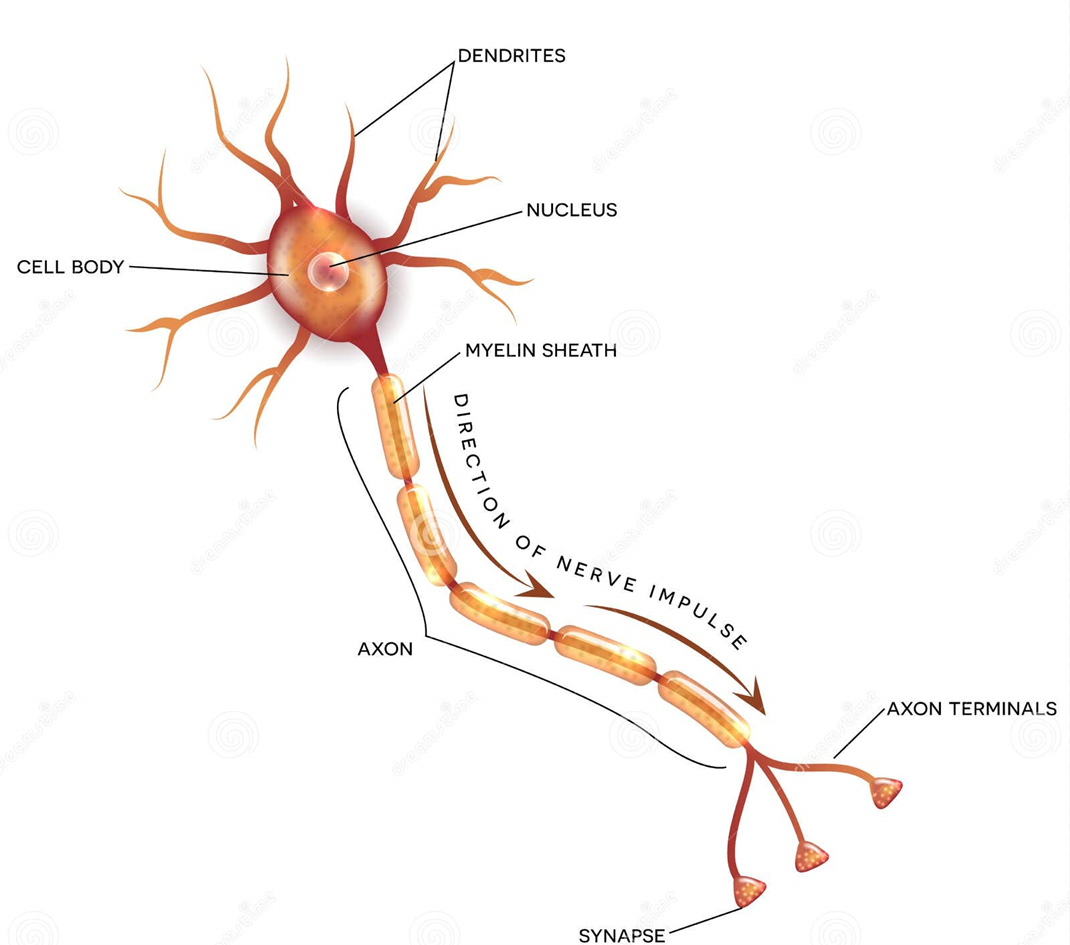
\includegraphics[width=0.5\textwidth]{Chapter2/Figs/2a.png}
\caption[Labeled diagram of the neuron.]{Labeled diagram of the neuron, nerve cell that is the main part of the nervous system. A neuron's dendrites include synapses that allow it to accept input from other neurons. The dendrites carry current to the soma, which is where electrical charge is integrated. If the neuron membrane gets sufficiently polarised, an action potential (also known as a spike) travels down the axon. This causes neurotransmitters to be released at synapses, resulting in currents in the dendrites of postsynaptic neurons.}
\label{fig:2a}
\end{figure}

\noindent Neurons represent only one of the numerous cell types within the brain, yet they are the most frequently discussed due to their status as the primary computational entities. Their fundamental function is relatively straightforward: neurons receive input from other neurons, and if that input is sufficiently stimulating, they will fire an action potential (also known as a spike), which propagates to other neurons.\\

\noindent Figure \ref{fig:2a} illustrates a basic cartoon of a neuron. Neurons can be subdivided into three principal parts: the dendrites, the cell body (soma), and the axon. Neurons receive input currents via their dendrites, which then transmit or channel this into the cell body, called the soma. When a neuron spikes, it sends current down its axon, which results in the release of neurotransmitter(s) at the synapses. These are connections from a neuron's axon to the dendrites of other neurons, and the neurotransmitter release causes dendritic input currents in these other connected neurons. \\

\begin{figure}[htbp!] 
\centering    
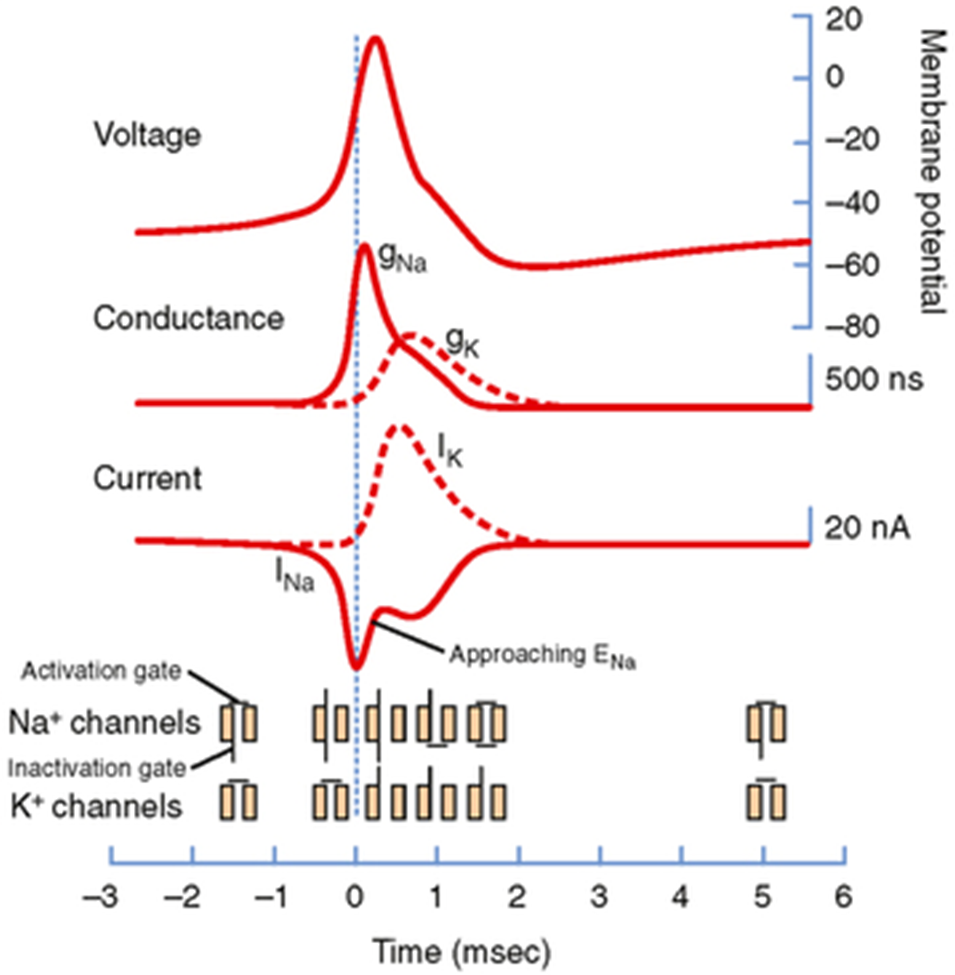
\includegraphics[width=0.45\textwidth]{Chapter2/Figs/2b.png}
\caption[Spiking dynamics of a neuron.]{The action potential and the underlying conductance and currents with respect to time \cite{squire2012fundamental}. It should be noted that the increased conductance for $Na^+$ (and its inward flow) is associated with the rising phase of the action potential, whereas the slower increase in conductance for $K^+$ (and its outward flow) is associated with repolarisation of the membrane and with afterhyperpolarisation. The reduction in $I_{Na}$ before the peak of the action potential (even though $G_{Na}$ is still high) is due to inactivation of the Na+ channels.}
\label{fig:2b}
\end{figure}

\noindent The soma represents the principal component of the neuron. From a computational perspective, the soma represents the integration point for all incoming currents from dendrites, marking the initiation of the action potential generation process (Figure \ref{fig:2b}). When a neuron is at rest, the soma exhibits a negative charge. This is referred to as the resting voltage and is maintained by ion pumps that regulate the concentration of ions (predominantly sodium, $Na^+$, potassium, $K^+$, and calcium, $Ca^{+2}$) within the cell. \\

\noindent As the currents arrive from the dendrites, they initiate a process of depolarisation of the cell. Once the voltage within the soma reaches a sufficient level, it initiates the opening of voltage-activated sodium channels, which permit the influx of sodium ions into the cell, further depolarising it. This process persists until the electrical gradient resulting from the accumulation of sodium ions reaches a point where it is no longer in equilibrium with the chemical gradient caused by the imbalance of sodium within and outside the cell. This leads to a notable increase in the neuron's positive charge, exceeding the resting voltage. \\

\noindent Furthermore, this substantial depolarisation also activates voltage-gated potassium channels, which subsequently permit the release of potassium ions from the cell, thereby facilitating repolarisation. Concurrently, the sodium channels undergo inactivation. The opening of potassium channels ultimately results in the cell reaching a voltage below its resting level, a state known as hyperpolarisation. The sodium channels remain inactivated and the potassium channels remain open for a period of time following the spike. \\

\noindent The combination of these factors renders it almost impossible for the neuron to fire during this time; this is referred to as the absolute refractory period. The change in ionic concentrations within the cell is relatively minor during a single spike, but over the course of numerous spikes, the ion pumps are required to maintain the optimal concentrations of sodium and potassium. Other currents, most notably calcium currents, are present in some neurons. \\

\noindent The rapid depolarisation associated with an action potential not only causes an increase in the somatic voltage potential, but also results in partial depolarisation of the axon segments situated in closer proximity to the soma. This results in the opening of sodium channels in that part of the axon, which in turn causes further depolarisation and the opening of sodium channels in the subsequent section of the axon. In this way, the somatic spike triggers a voltage wave that travels down the axon, eventually leading to the release of neurotransmitter(s) from synaptic vesicles situated near the ends of the axon. \\

\noindent Axons are responsible for transmitting long-range signals in the brain, and thus exhibit considerable variation in length, contingent on whether a given neuron is connected to neighbouring neurons or to neurons situated in a different brain region. To facilitate long-range transmission, axons are coated in myelin, a substance composed mainly of lipids and thus a good electrical insulator. This enables the propagation of current down the axon. The high proportion of fat makes myelin white; bundles of axons are responsible for the "white matter" parts of the brain. In contrast, the "grey matter" is composed mainly of neuron dendrites, somas, and short-range axons \cite{mel1994information}.\\

\noindent Dendrites are thin processes that extend away from the soma to connect to the axons of other neurons \cite{johnston1996active}. They serve to transmit current from synapses with other neurons to the soma. Initially, it was thought that they only conducted current passively; however, research has demonstrated that they possess active conductance mechanisms that are analogous to those involved in spike generation and propagation down an axon.\\

\noindent Dendrites are also traditionally considered to act in a linear manner, whereby inputs from numerous synapses are accumulated over time and space. This remains a prevalent assumption in numerous computational models. However, recent studies have demonstrated that the summation of signals in dendrites is more intricate, exhibiting a combination of linear and nonlinear (sigmoidal) elements \cite{polsky2004computational}.\\

\noindent Neurons are connected to one another by synapses, which facilitate the connection between the axon of the presynaptic neuron and a dendrite of the postsynaptic neuron. Upon the occurrence of a spike in the presynaptic neuron, an electrical pulse is transmitted along the axon, reaching the presynaptic terminals of all synapses situated along its length. The synaptic vesicles, which are filled with neurotransmitter, are located at the terminals. \\

\noindent When an electrical pulse is generated, it causes the vesicles to release neurotransmitter into the synaptic cleft, which is the narrow space between the presynaptic terminal and the postsynaptic terminal. This neurotransmitter then activates receptors on the postsynaptic terminal, which open and permit the flow of current into the postsynaptic cell. The specific neurotransmitter utilized by the synapse is contingent upon the presynaptic neuron. \\

\noindent All synapses on a neuron's axon release the same neurotransmitter or combination of neurotransmitters, a phenomenon known as Dale's principle. At the time of its development, Dale's principle was based on the assumption that each neuron produced a single type of neurotransmitter. However, evidence of cotransmission was only discovered in 1976 \cite{burnstock2004cotransmission}, with the understanding that neurotransmitters can be excitatory or inhibitory. It is not the case that any neurons play both an excitatory and inhibitory role with respect to different postsynaptic cells. \\

\noindent A significant proportion of the most influential findings in computational neuroscience are based on mathematically detailed models of neuronal functioning. One of the most renowned of these is the Hodgkin-Huxley model of the squid giant axon \cite{hodgkin1952quantitative}. In recent times, the number of available neuron models has proliferated. \\

\noindent The models currently in use in the literature range from the simplest possible rate-neuron model, namely binary threshold units \cite{stocks2001information}, to complex multi-compartmental models that account for detailed dendritic morphologies \cite{markram2015reconstruction}. In the context of large-scale neural models aiming to reproduce high-level behaviours, single-compartment neuron models remain the prevailing approach. \\

\noindent These models treat the neuron as a single electrical compartment, combining the dendrites, soma, and axon. In contrast, multi-compartmental models represent the neuron as comprising multiple electrical compartments, with equations that describe the influence of activity in one compartment on that of another. \\

\noindent The number of compartments in a model can vary considerably, from a minimalistic two-compartment structure, typically comprising one for the dendrites and one for the soma, to a more elaborate configuration comprising thousands of compartments. The number of compartments in a model is directly proportional to the amount of computing power required for simulation and the complexity of the resulting behaviour. For these reasons, models that seek to reproduce behaviour predominantly utilise either single-compartment neurons or simpler models that do not model the electrical activity of the neuron at all. \\

\noindent Single-compartmental neuron models can be classified according to two key dichotomies: firstly, the rate-based versus spike-based dichotomy; and secondly, the static versus dynamic dichotomy. The distinction between rate-based and spiking neuron models concerns the nature of the output: is it a continuous value, represented by a firing rate, or a discrete value, represented by a spike.\\

\noindent The majority of neurons in the mammalian cortex communicate via spikes, making spiking neuron models more physiologically realistic. However, there are limited areas in the mammalian brain, such as horizontal cells in the retina, where neurons communicate via gap junctions, potentially transmitting a continuous value rather than a discrete spike. \\

\noindent The distinction between static and dynamic models concerns the extent to which the model exhibits internal dynamics. In a static model, the output at a given point in time is independent of the neuron's past history and solely contingent on its instantaneous input. In contrast, a dynamic model allows for some degree of dependence on the neuron's past trajectory.\\

\noindent Dynamic neuron models possess a state, which is to say, internal variables that evolve over time and are not directly computable from the present input to the model. They are typically expressed using differential equations. In contrast, static models output a function of the current input only; thus, they do not require differential equations to express them. \\

\noindent It is important to note that the distinction between static and dynamic neurons does not necessarily refer to whether the neuron is being used as a static nonlinearity, evaluated at a single point in time on an input value, or as a dynamic nonlinearity, evaluated over a period of time on an input signal. \\

\noindent Static neurons can be evaluated dynamically by evaluating them independently at each successive point in time on the input value. In contrast, there is no general method for evaluating dynamic neurons statically, as their input at any given point in time is contingent upon their internal state, which is a dynamic process that evolves over time. \\

\noindent In some cases, it is possible to determine a firing rate response curve, also known as an I-F response curve or rate response function, for dynamic neuron models. This curve maps every constant value of the input current to a constant firing rate output. This can be determined analytically or empirically by applying a constant input current and measuring the rate of the output spikes, this can even be done in real neurons in vitro. \\

\noindent However, many neuron models will not output spikes at a constant rate, even for a constant input, due to changing internal dynamics. In such cases, the rate-response function only captures part of the model, and will be different depending on the state of the model and how it is measured or calculated. \\

\begin{table}
\caption{Neuron Model Dichotomies.}
\centering
\begin{tabular}{|c|c|c|}
\hline
                 & \textbf{Rate}                                                                  & \textbf{Spiking}                                             \\ \hline
\textbf{Static}  & Sigmoid Rate LIF                                                               & Poisson Spiking                                              \\ \hline
\textbf{Dynamic} & \begin{tabular}[c]{@{}c@{}}Adaptive Rate LIF\\ Sigmoid with State\end{tabular} & \begin{tabular}[c]{@{}c@{}}Hodgkin-Huxley\\ LIF\end{tabular} \\ \hline
\end{tabular}
\label{table:4a}
\end{table}

\noindent Table \ref{table:4a} illustrates the manner in which a small selection of neuron models align with these dichotomies. In the static rate category, the models in question take in a continuous value and output a continuous function of that value. This encompasses the majority of non-linearities employed in machine learning (such as sigmoids or rectified linear units), in addition to the analytic firing rate for the LIF neuron model. \\

\noindent In the static spiking category, models are characterised by the output of a discrete (binary) function of their continuous input. This category is primarily composed of Poisson-spiking neurons, which fire probabilistically based on their instantaneous firing rate. This implies that the probability of firing at a given time is independent of past firings. Furthermore, Poisson spiking can be applied to a dynamic rate model, whereby the probability of spiking is independent, but the spike rate is a dynamic process. \\

\noindent Dynamic rate models possess an internal state that influences their continuous output, in addition to the input. This encompasses the analytic LIF rate model with adaptation, which possesses an intrinsic adaptation parameter that increases when the neuron is active and discounts the firing rate. Furthermore, the category encompasses sigmoid neuron models that possess an underlying voltage that is dynamically correlated with the neuron inputs \cite{lillicrap2016random}. \\ 

\noindent The dynamic spiking category also includes the LIF neuron model, the Hodgkin-Huxley model, and more intricate multi-compartmental models. Within the category of spiking models, a distinction can be made between those that output instantaneous spikes (e.g., LIF) and those that output spikes that vary across time (e.g., Hodgkin-Huxley). Recently, another study have employed such models in the context of deep networks \cite{guerguiev2017towards}, subject to biological constraints. \\

\noindent Another potential distinction can be made between models that output stereotyped spikes, where the size of each spike is identical, and those that output variable-sized spikes. Models of cortical neurons that output instantaneous spikes (e.g., LIF) almost invariably output stereotyped spikes. This is due to the fact that spikes in cortical neurons are almost identical in terms of magnitude, duration, and shape.\\

\noindent It is widely believed that none of these factors carry information. Even among models that have spikes that vary across time (e.g., Hodgkin-Huxley), the spike magnitude, duration, and shape are quite consistent between spikes. Therefore, the majority of spiking cortical neuron models exhibit stereotyped spikes. \\

\noindent By modelling the spike separately from the rest of the neural dynamics, it is possible to separate time scales, thereby avoiding the need for additional computational resources to model the spike trajectory, which is characterised by stereotyped details of little interest \cite{abbott1999lapicque}. \\

\subsection[Neuron Models]{Neuron Models}

\begin{figure}[htbp!] 
\centering    
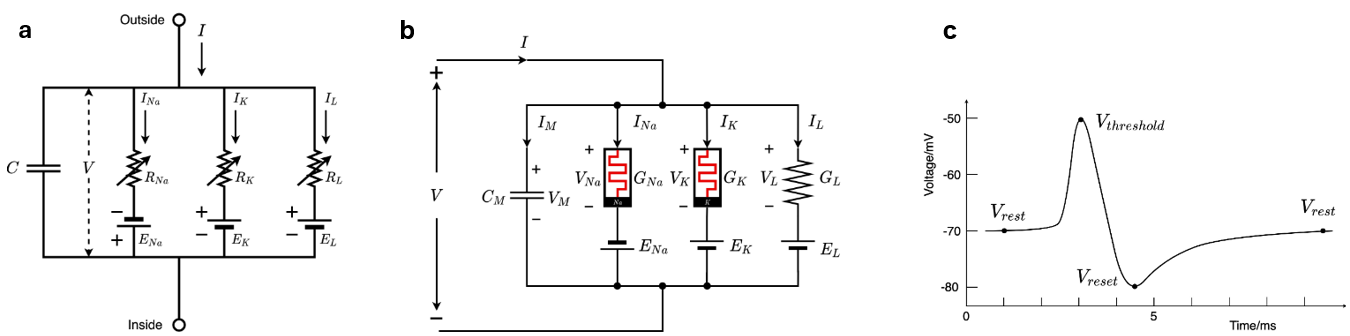
\includegraphics[width=1\textwidth]{Chapter2/Figs/2c.png}
\caption[Hodgkin-Huxley neuron model.]{Hodgkin-Huxley neuron model. (a) An equivalent circuit for the HH models \cite{hodgkin1952quantitative}. (b) An equivalent circuit for memristive HH model \cite{chua2012hodgkin}. (c) An action potential waveform, which demonstrates the resting, threshold, and reset potentials. }
\label{fig:2c}
\end{figure}

\noindent A variety of neuron models have been developed to describe the complex dynamics of biological neurons. Among these, the Hodgkin–Huxley (HH) model is one of the most widely used, comprising a set of nonlinear differential equations that accurately approximate the electrical signals of neurons. \\

\noindent Figure \ref{fig:2c}(a) depicts the HH neural model, wherein the time-varying nonlinear conductor $R_{Na}(GNa)$ and $R_K(G_K)$ represent the sodium and potassium channels, respectively, while the linear conductor $R_L(G_L)$ simulates leak channels and $C$ models the membrane of a neuron. The equations of the HH model are presented below: 
\begin{align}
C \frac{dV_m(t)}{dt} = I_C(t) + \sum_{k}^{}I_k(t) \label{eq:2.1} 
\end{align}

\noindent In this context, $V_m$ represents the membrane potential. $\sum_{k}^{}I_k(t)$ denotes the sum of the ionic currents flowing into the neuron. This can be formulated by three ion currents, as follows:
\begin{align}
\sum_{k}^{}I_k &= C_m \frac{dV_m}{dt} + G_Kn^4(V_m - V_K) + G_{Na}m^3(V_m - V_{Na}) + G_L (V_m - V_L) \label{eq:2.2} \\
\frac{dn}{dt} &= \alpha_n(V_m)(1-n)-\beta_n(V_m)n \label{eq:2.3} \\
\frac{dm}{dt} &= \alpha_m(V_m)(1-m) - \beta_m(V_m)m \label{eq:2.4} \\
\frac{dh}{dt} &= \alpha_h(V_m)(1-h)-\beta_h(V_m)h \label{eq:2.5}
\end{align}

\noindent The reversal potentials $V_K$, $V_{Na}$, and $V_L$ are the three parameters in question. The rate constants $\alpha_i$ and $\beta_i$, which depend on the membrane potential, describe the behaviour of the $i^{th}$ ion channel. The maximal value of the conductance is represented by $G_K$, $G_{Na}$, and $G_L$. Finally, the dimensionless quantities \textit{n}, \textit{m}, and \textit{h}, which lie between 0 and 1, are associated with three ion channels. \\

\noindent In order to achieve the optimal fit for human cardiac action potentials, the HH model is reduced by setting the leakage channel conductance to $G_L = 0$  \cite{noble1962modification}.It has been demonstrated that $G_{Na}$ and $G_K$ are memristors \cite{chua1976memristive}, as illustrated by the equivalent circuit in figure \ref{fig:2c}(b). \\

\noindent The integrate-and-fire (IF) neuron \cite{lapicque1907louis} constituted one of the earliest computational models of a neuron. This model was developed prior to the ability of researchers to measure the electrical and chemical changes occurring in a functioning neuron. It is based on the premise that the neuron membrane can be modelled as a capacitor that stores charge over time \cite{abbott1999lapicque}.\\

\noindent As the name suggests, the IF model exhibits two principal behaviours: The model integrates current over time, as would be expected of a capacitor, and fires when the voltage reaches a threshold. Furthermore, the model may or may not incorporate a leak term, which represents a resistor in parallel with the capacitor that permits the dissipation of charge over time. \\

\noindent The model with a leak term is typically designated as the leaky integrate-and-fire (LIF) model. While the term "integrate-and-fire (IF) model" can be applied to either the leaky or non-leaky model, in this thesis it will be used to refer specifically to the non-leaky version of the model. \\

\noindent With the objective is to identify how the neuron's membrane voltage evolves over time and, based on this, to determine when the neuron spikes. The charge \textit{Q} across a capacitor is given by $Q = V \times C$, where \textit{V} is the voltage across the capacitor and \textit{C} is the capacitance. Differentiating this with respect to time, we find that the membrane voltage $\textit{V(t)}$ of the neuron is governed by:
\begin{align}
C \frac{dV(t)}{dt} = J(t) \label{eq:2.6} 
\end{align}

\noindent In this context, \textit{J(t)} represents the input current to the neuron over time, whereas \textit{C} denotes the membrane capacitance. It should be noted that current is the time derivative of charge. Equation \ref{eq:2.6} demonstrates that the IF neuron simply integrates the input current over time. It is still necessary to identify the point at which the neuron spikes. \\

\noindent This is achieved by defining a threshold voltage, $V_{th}$, which is exceeded when the voltage passes this threshold, resulting in the neuron firing. This is a fundamental principle in neurophysiology: once the neuron voltage passes a threshold, the neuron begins firing a spike, and once this firing process begins, it is almost impossible to reverse. \\

\noindent A reset procedure is finally defined. Once a neuron has fired a spike, the membrane voltage is reset to the resting potential, $V_{rest}$. This phenomenon can be attributed to physiological processes. Following the occurrence of a spike in a neuron, other ionic currents, typically potassium, are initiated, leading to a restoration of the membrane voltage towards the resting potential.\\


\noindent Some integrate-and-fire models may also incorporate an absolute refractory period, defined as a time interval during which the voltage is maintained at the resting potential $V_{rest}$ following a spike. In cortical neurons, post-spike potassium currents are sufficiently strong to prevent another spike from occurring for a considerable duration. This time interval is referred to as the absolute refractory period. The model accounts for this by holding the membrane voltage at $V_{rest}$ for a duration equal to the absolute refractory period. \\

\noindent The leaky integrate-and-fire (LIF) model \cite{knight1972dynamics} incorporates an additional physiological factor: Neuron membranes are not perfect capacitors; rather, they slowly leak current over time, pulling the membrane voltage back to its resting potential. Therefore, the membrane is modelled as a capacitor and resistor in parallel, which allows for the neuron to exhibit a degree of "forgetting": in the absence of any input, the membrane voltage will return to its resting potential \cite{koch2004biophysics}. The LIF dynamics are captured by the following equation:

\begin{align}
C \frac{dV(t)}{dt} = J(t) - \frac{1}{R} (V - V_{rest}) \label{eq:2.7} 
\end{align}

\noindent In this model, \textit{R} represents the membrane resistance, and the remaining parameters are consistent with those of the IF model. The resetting procedure is also identical to that of the IF model.\\

\noindent The LIF model comprises a number of parameters, including $C, R, V_{rest}$ and $V_{th}$. It is possible to normalise the model in order to reduce the number of parameters while maintaining the full dynamics of the original model. In particular, the model can be manipulated so that the normalised voltage lies within the range [0, 1], with a normalised resting potential of zero and a normalised firing threshold of one. Initially, Equation \ref{eq:2.7} is multiplied by R to give:

\begin{align}
\tau_{rc} \frac{dV}{dt} &= RJ(t) - V + V_{rest} \label{eq:2.8} \\
\tau_{rc} &= R \times C \label{eq:2.9} \\
\bar{V} &= \frac{V - V_{rest}}{V_{th} - V_{rest}} \label{eq:2.10} \\
\bar{V_{rest}} &= \frac{V_{rest}}{V_{th}} \label{eq:2.11} 
\end{align}

\noindent By substituting $\bar{V}$ and $\bar{V_{rest}}$ into equation \ref{eq:2.3} to give:


\begin{align}
\tau_{RC}(V_{th} - V_{rest})\frac{d\bar{V}}{dt} &= RJ(t) - \bar{V}(V_{th} - V_{rest})
 \label{eq:2.12} \\
\tau_{rc}\frac{d\bar{V}}{dt} &= \frac{R}{V_{th} - V_{rest}} J(t) - \bar{V} \label{eq:2.13} \\
\tau_{rc} \frac{d\bar{V}}{dt} &= \bar{J}(t) - \bar{V} \label{eq:2.14} 
\end{align}

\noindent When the firing threshold for the new equation $\bar{V_{th}} = 1$, the voltage resets to $\bar{V_{rest}} = 0$, and $\bar{J}(t) = \frac{R}{V_{th} - V_{rest}} J(t)$. It can be observed that $\bar{J}(t)$ is merely a linear transformation of $J(t)$. Consequently, Equation \ref{eq:2.14} retains the full dynamics of Equation \ref{eq:2.7} for a scaled input, but with only one parameter, $\tau_{RC}$. \\

\noindent It should be noted that both $\bar{V}$ and $\bar{J}$ are unitless quantities. Conventionally, the unitless space is employed exclusively, and the quantities are often referred to simply as \textit{V} and \textit{J}, despite the fact that they are not voltages or currents. This simplifies the mathematical representation, without limiting the generality of the models. \\

\noindent Equation \ref{eq:2.14} provides an exact description of the circumstances under which the model neuron will spike in response to a given input current, \textit{J(t)}. However, in some cases, it is sufficient to consider only the spike rate, that is, the number of spikes per second that the neuron will produce in response to a given input current. \\

\noindent In the case of the LIF model, it is possible to determine the analytical firing rate for a constant input current. This is achieved by calculating the inter-spike interval (ISI), which is the time between one spike and the next. The firing rate is then given by the inverse of the ISI. When a constant input current, $J(t) = j$, is provided, it is possible to solve Equation \ref{eq:2.14} in order to find the neuron voltage over time. 
\begin{align}
V(t) = (V(0) - j)e^{\frac{-t}{\tau_{rc}}} + j \label{eq:2.15}
\end{align}

\noindent In the absence of spikes, the objective is to ascertain the time required for the voltage to increase from$ V(0) = 0$ to $V(t) = 1$. This property will only occur if $j > 1$. Substitution into Equation \ref{eq:2.15} and subsequent solution for \textit{t} yields:
\begin{align}
t = - \tau_{RC} log \left( - \frac{1}{j} \right) \label{eq:2.16}
\end{align}

\noindent Incorporating the refractory period and performing the inversion, the spike rate \textit{r} for the LIF neuron is given by:
\begin{align}
r &= \begin{cases}
\frac{1}{t_{ref} - \tau_{RC} log \left( 1 - \frac{1}{j} \right)} & \text{ if } j > 1 \\ 
0 & \text{ otherwise }  
\end{cases} \label{eq:2.17}
\end{align}

\noindent The LIF model is one of the most widely utilised simplified neuron models \cite{lapique1907researches}. The simple equivalent model is illustrated in Figure \ref{fig:2d}(a). In this model \cite{stein1967frequency}, a resistor \textit{R}, connected in series with a \textit{DC} source $V_{rest}/V_{reset}$, is connected in parallel with a capacitor \textit{C}. A postsynaptic neuron receives a synaptic current \textit{I(t)}, generated by presynaptic spikes. \\

\noindent A proportion of the current \textit{I(t)} flowing into \textit{C} results in an increase in the membrane potential \textit{V(t)}. The charge leakage occurs via resistor \textit{R}. When \textit{V(t)} reaches a threshold value, the neuron generates a spike. Following the generation of a spike, the membrane potential is reset to the reset value. \\

\noindent In the absence of \textit{I(t)}, the voltage across \textit{C} is eventually settled at $V_{rest}$, representing the cell's resting potential. During the refractory period $t_0$, a neuron is incapable of spiking. Figure \ref{fig:2d}(c,d) illustrates the LIF neuron dynamics for the case of a \textit{DC} input current and a zero rest and reset potential, $E_{reset} = E_{rest} = 0$ \cite{tal1997computing}. \\

\begin{figure}[htbp!] 
\centering    
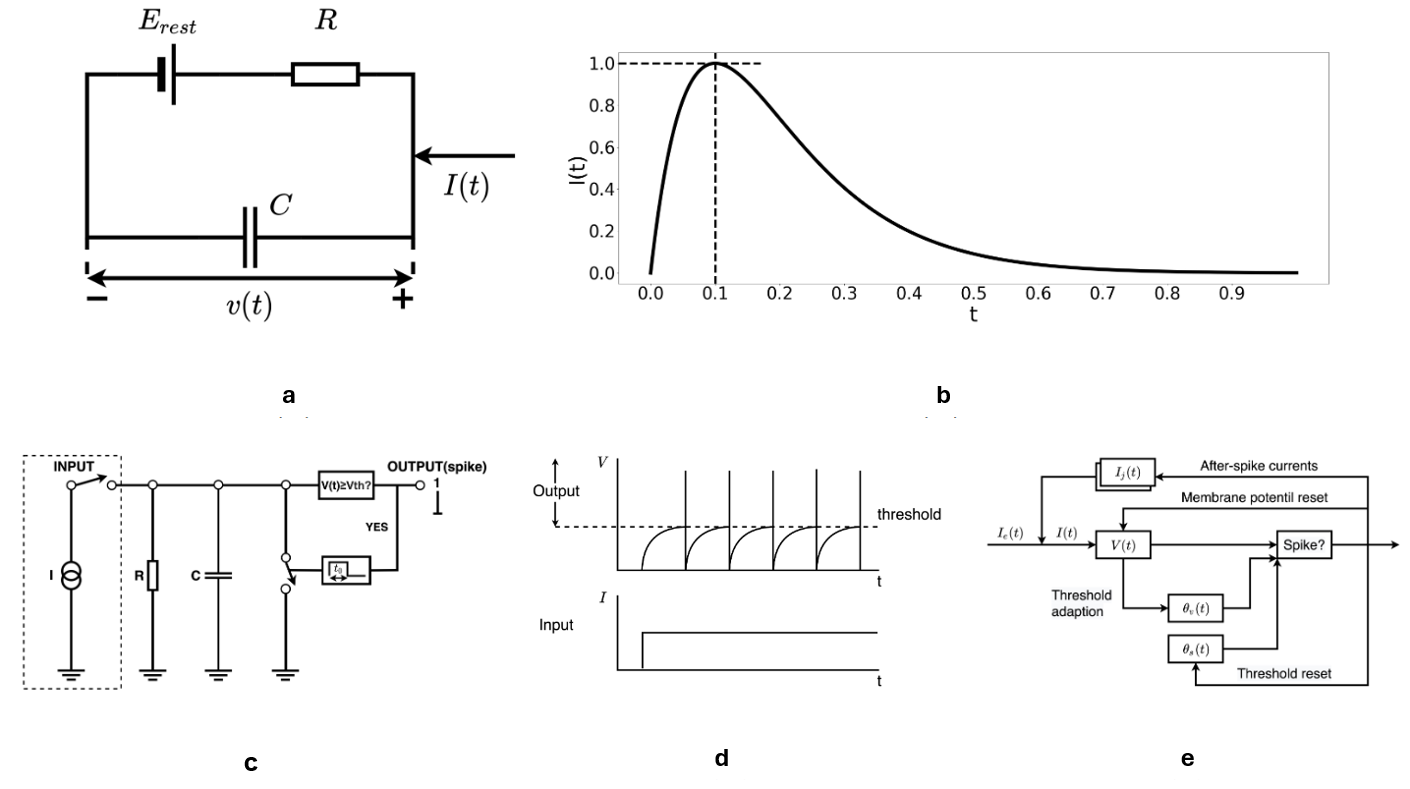
\includegraphics[width=1\textwidth]{Chapter2/Figs/2d.png}
\caption[The Leaky Integrate-and-Fire neuron model.]{The LIF neuron model. (a) Schematic diagram of the LIF electrical model. (b) Input current in the form of an alpha function, $\tau_{\alpha} = 0.1, I_0 = 1$ (c)The LIF model allows for the control of spiking behaviour through a comparison of membrane potential and threshold at each time step. Upon the triggering of a spike, a voltage-controlled switch discharges C for a duration corresponding to the refractory period $t_0$ \cite{tal1997computing}. (d) A simulation of constant firing frequency for DC current input in which $t_0$ is hidden. DC input current and output spikes are both shown. (e) A generalised LIF model with threshold control \cite{teeter2018generalized}. }
\label{fig:2d}
\end{figure}

\noindent The input synaptic current, \textit{I(t)}, can be described by a time-varying alpha function. However, alternative functions may be employed, including "Instantaneous Rise and Single Exponential Decay," "Biexponential Functions," "Sawtooth," and "Pulse Function." The alpha synaptic current is modeled by Equation \ref{eq:2.15}, and the resulting plot is shown in Figure \ref{fig:4b}(b). \\

\noindent Nevertheless, Figure \ref{fig:2d}(a) lacks a circuit for resetting the system when the threshold is reached. In order to evaluate the inequality $V > V_{threshold}$, it is necessary to use an active circuit, such as a comparator. Upon reaching the threshold, the membrane potential must be reset in accordance with the illustration in Figure \ref{fig:2d}(d). Therefore, the LIF model's generalized version necessitates additional overhead, as illustrated in Figure \ref{fig:2d}(e). \\

\noindent In the generalized LIF model, the reset behavior necessitates external control to pull down the membrane potential below the resting potential. This external control requires intricate, active circuits comprising MOS transistors, resistors, and even a silicon-controlled rectifier (SCR), which represents a significant drawback in a neuromorphic system due to its substantial power and area consumption. \\

\noindent In order to address the limitations of conventional neuron models, memristor technologies can be employed to emulate biological neurons with the objective of reducing energy consumption and increasing packing density. The HH model has been emulated by utilising two memristors in parallel with two capacitors, respectively mimicking two channels that are coupled to each other with a resistor. \\

\noindent Additionally, an input resistor and an output impedance comprising a resistor and a capacitor have been proposed \cite{pickett2013scalable}. The LIF neuron has been demonstrated using a diffusive/volatile memristor in parallel with a capacitor, and the neuron has been employed in a fully memristive neural network \cite{wang2018fully}. \\

\noindent Despite the existence of memristor-based neuron models, the lack of accessible experimental data and hardware for prototyping memristive circuits represents a significant obstacle. A significant number of state-of-the-art experimental demonstrations have relied on bespoke fabrication processes that cannot be reproduced using off-the-shelf memristors. \\

\noindent Furthermore, the limited choice of commercially available, low-cost, discretely packaged memristors, which are known to be highly sensitive and stochastic in behaviour, has compounded the issue. The challenge in developing hardware prototypes has made it difficult to perform experimental validation. \\

\noindent In addition to the acceleration of neural networks, the design of a solid-state brain that can harness the neural code has gained increasing attention as a means of processing vast quantities of sensory data without being constrained by the von Neumann bottleneck. The solid-state brain is structured in a manner that emulates the cerebral cortex, with neurons interconnected by a vast array of variable synapses. \\

\noindent It is hypothesised that neurons and synapses can be realised with memristors integrated with a complementary metal-oxide semiconductor (CMOS) process. However, the design of a large-scale solid-state brain remains elusive in neuromorphic computing due to the considerable overheads associated with mimicking the surface area of neural tissue, constrained power consumption, routing, and the massive parallelism of synaptic connections.

\subsection[Synapse Models]{Synapse Models}

Prior to model internal neural dynamics, it is essential to model the dynamics of the synapses that connect neurons to one another. Synapses exert a significant functional effect as a low-pass filter on the spikes that pass through them. A spike in the presynaptic neuron elicits an extended current pulse in the postsynaptic neuron. This pulse can be conceptualised as a low-pass filtered version of the presynaptic spike. \\

\noindent The simplest model of a synapse is that of a first-order low-pass filter. The impulse response of a filter describes the manner in which the filter responds to an infinitesimally short input of unit integral, which is called an impulse. This idealised impulse is also a reasonable model of a spike, and thus the impulse response also describes what the postsynaptic current will look like in response to a presynaptic spike. The impulse response of the first-order low-pass filter is as follows:
\begin{align}
h(t) = \frac{1}{\tau_s}e^{\frac{t}{\tau_s}} \label{eq:2.18} 
\end{align}

\noindent The synaptic time constant, denoted by $\tau_s$, is defined as the length of time over which the postsynaptic current is spread. Given that the impulse response is an exponential function, the exponential synapse model is therefore a suitable description.
\begin{align}
h(t) = \frac{1}{\tau_s^2}e^{\frac{t}{\tau_s}} \label{eq:2.19} 
\end{align}

\noindent It was determined that a second-order lowpass filter is a superior model for a synapse \cite{mainen1995reliability}. The impulse response of this filter is defined by the 
equation \ref{eq:2.19}. This function is referred to as the alpha function, and thus the model is designated as the alpha synapse model. Both of these models are based on the current generated by a spike in the postsynaptic neuron, which is a current-based synapse model.\\

\noindent Other current-based synapse models exist; a popular one is the double-exponential model, which is similar to the alpha synapse but with two time constants, thereby affording greater control over the rise and fall of the impulse response. Where The double-exponential model with both time constants set to the same value reduces to the alpha synapse. \\

\noindent Many of the other, more realistic synapse models are conductance-based, meaning that they model the conductance of the neural membrane at the synapse. The current flowing into the neuron is dependent on both the conductance and the voltage across the membrane. The latter undergoes a change as the synapse becomes active. \\

% \subsection[Neural Coding Schemes]{Neural Coding Schemes}

\noindent One of the primary objectives of computational neuroscience is to ascertain the manner in which the brain represents—or encodes—information. To this end, researchers have put forth a multitude of potential coding schemes that neurons could utilise for information encoding. One key distinction between rate coding and temporal coding is the following dichotomy. \\

\noindent In a rate code, the sole pertinent measure is the firing rate (i.e. the number of spikes) of a neuron over a given period of time. An exemplar of a rate code is motor neurons in the peripheral nervous system. The contraction of a muscle is contingent upon the number of spikes per unit time; thus, only the rate of motor neuron spikes is significant \cite{gerstner1997neural}. In a temporal code, the time of individual spikes is also a factor. An exemplar of a timing code is the early auditory system, where precise spike timing facilitates the localisation of sounds \cite{chase2006spike}.\\

\noindent The precise definitions of rate and temporal codes remain contentious, with differing interpretations presented by various authors \cite{dayan2005theoretical}. To illustrate, a neuron may discharge a number of spikes in rapid succession, followed by a period of quiescence. A second neuron may be observed to fire the same number of spikes, but in a more evenly distributed manner over a given period. \\

\noindent One possible interpretation is that both neurons have the same firing rate, but the first has all its spikes occurring near the beginning of the period, in which case the timing of the spikes is a significant factor. An alternative perspective posits that the instantaneous firing rate of the first neuron fluctuates over the period, whereas that of the second neuron remains constant. This suggests that it is the instantaneous firing rate, rather than the overall firing rate, that is of primary importance. \\

\noindent This highlights a limitation of solely examining the overall firing rate (i.e., the number of spikes) of a neuron over a given period. It is unclear which period should be considered. In real neurons, the period of time that is relevant for counting spikes depends on parameters such as the membrane time constant tau of the postsynaptic neuron. \\

\noindent For this reason, neuroscientists will often differentiate between rate and timing codes based on the frequency of alterations in the instantaneous firing rate. If the rate of firing exhibits rapid fluctuations, and if these fluctuations contain information about the stimulus (and are not simply spurious variation or "noise"), then the code is said to be temporal; otherwise, it is a rate code. \\

\noindent Once again, there is a lack of consensus regarding the minimum frequency of fluctuations in firing rates that must be observed to qualify as temporal codes. One possible definition is relative to the stimulus. The firing rate of neurons can be triggered to change rapidly in response to fast-changing stimuli, regardless of whether the code in use is rate or temporal. \\

\noindent If the temporal code is defined as having meaningful firing rate fluctuations at a faster time scale than changes in the stimulus, then it can be differentiated between codes that have fluctuations because they are using them for coding and those that simply have fluctuations triggered by the stimulus. According to this definition, neurons using a temporal code will have a fluctuating firing rate in response to a constant stimulus, whereas neurons using a rate code will have a non-fluctuating firing rate. \\

\noindent Both rate codes and temporal codes describe the encoding properties of individual neurons. Additionally, one may inquire about the coding properties of a group (also known as a population) of neurons. The concept of population coding pertains to instances where a representation is distributed across numerous neurons within a population, such that the represented value cannot be decoded from the activities of a limited number of neurons.\\

\noindent To illustrate, the simplest method of extrapolating the concept of rate or temporal coding to multiple neurons would be to have numerous neurons all implementing the same code. In other words, all neurons will exhibit a similar firing pattern when representing a given value, due to their comparable tuning properties. This results in a significant degree of redundancy between neurons. \\

\noindent In contrast, population coding entails each neuron representing a distinct aspect of the represented value. To illustrate, if the objective is to represent head direction, there are neurons that represent a head that is fully turned to the left, others that represent a head that is fully turned to the right, and still others that represent a centred head. Additionally, there are neurons that represent values in between these three head directions. The direction in which a neuron is most active is referred to as its preferred direction. \\

\noindent It should be noted that each neuron exhibits some degree of variance, whereby it will fire for head directions that are relatively close to its preferred direction. Conversely, the further the actual head direction is from a neuron's preferred direction, the less it will fire. By utilising the activities of all neurons in the population, it is possible to decode the head direction with a high degree of accuracy. \\

\noindent From a population perspective, it is possible to differentiate between codes that exploit synchrony between neurons and those that do not. This can be facilitated, for example, by coincidence detection, whereby a postsynaptic neuron will only fire if the spikes of two of its input neurons are coincident, that is to say, they fall within the same (small) temporal window. \\

\noindent This distinction between temporal and rate coding schemes is further exemplified by the fact that only temporal codes can take advantage of correlations between individual spikes of neurons. Rate coding schemes, on the other hand, can only take advantage of synchrony between neurons in terms of synchronised fluctuations of their instantaneous firing rates, since they lack the temporal precision to co-ordinate individual spikes.

\section[Methodology]{Methodology}

\subsection[Modified Device Stack]{Modified Device Stack}

A distinct set of devices with disparate top electrical contacts were characterised, one with conductive indium tin oxide (ITO) in lieu of gold. The bottom contact and oxide layer remained unaltered and consistent with those observed in the gold-contacted devices presented in the preceding section. When subjected to stress, the ITO-contacted device exhibited a distinct response compared to the gold-titanium contacted device. Instead of a gradual and smooth increase in conductance, the response was more erratic and chaotic. \\

\begin{table}[h]
\caption{Comparison of the modified device stacks.}
\centering
\begin{tabular}{|cc|cc|}
\hline
\multicolumn{2}{|c|}{Original Stack}              & \multicolumn{2}{c|}{Modified Stack}              \\ \hline
\multicolumn{1}{|c|}{Layer} & Film Thickness (nm) & \multicolumn{1}{c|}{Layer} & Film Thickness (nm) \\ \hline
\multicolumn{1}{|c|}{Au}    & 110                 & \multicolumn{1}{c|}{ITO}   & 30                  \\ \hline
\multicolumn{1}{|c|}{Ti}    & 3                   & \multicolumn{1}{c|}{Ti}    & 3                   \\ \hline
\multicolumn{1}{|c|}{SiOx}  & 35                  & \multicolumn{1}{c|}{SiOx}  & 20                  \\ \hline
\multicolumn{1}{|c|}{Mo}    & 280                 & \multicolumn{1}{c|}{Mo}    & 150                 \\ \hline
\end{tabular}
\end{table}

\noindent The aluminium-contacted devices have yet to demonstrate the occurrence of current transients following the application of stress. In addition to failing to exhibit current transients, any increase in conductance induced by the constant current stress is also observed to be more volatile than that observed in the other devices, with the devices returning to a high resistance state within a couple of hours.\\

\begin{figure}[htbp!] 
\centering    
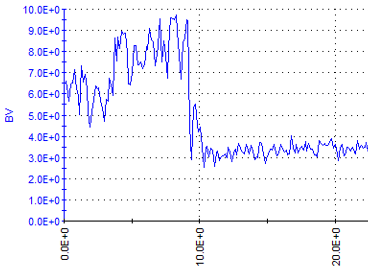
\includegraphics[width=0.5\textwidth]{Chapter2/Figs/2e.png}
\caption[Stressing responses of ITO top contacted device.]{Stressing responses of ITO top contacted device. With the objective to ascertain the stress responses of the ITO top-contacted device, the voltage across the device was monitored while it was subjected to a constant current of $-0.5\mu A$. It was not possible to apply larger currents. The response was observed to be less smooth when compared to that of the gold-contacted device.}
\label{fig:2e}
\end{figure}

\noindent In contrast, the ITO contacted devices did exhibit transients, but interestingly, only partially. A typical transient observed in ITO devices is plotted in Figure \ref{fig:2e}. It exhibits the initial increase in conductance as is typical with current transients, but does not then start reducing in conductance. Instead, the device exhibits a chaotic spiking-like behaviour which, if observed for too long, will cause the device to switch to a low resistance state.\\

\noindent The observation of a partial current transient in ITO-contacted devices is a significant finding. As will be discussed in the following section, this evidence is indicative of the transient being the result of multiple simultaneous changes occurring in the device. Furthermore, it supports the hypothesis that the top metal-insulator interface plays a role in generating transients.\\

\noindent The hypothesis that alterations to specific interfaces of the device can influence the characteristics of the current transient is supported by findings in tantalum oxide-based devices \cite{tuller2011point}. In this study, a layer of $Al_2O_3$ was deposited between the tantalum oxide bulk and the titanium nitride electrodes, which reduced the prominence of the current transient in the absence of the buffer layer.\\

\noindent To illustrate, the gradual decline in conductance of the transients is exclusive to the gold-contacted device, indicating that it is either due to the characteristics of the metal-insulator interface or the disparate responses to stressing at this interface that determine whether the decaying behaviour is manifested. \\

\noindent In contrast, the initial increase in conduction is observed in both the ITO and gold-contacted devices. This suggests that the behaviour is less affected by the top metal-insulator interface and may be located in the bulk oxide layer or at the bottom metal-insulator interface. The disappearance of the slower decay in conductance with the change in top electrode may provide insight into the physical model describing the current change. 

\subsection[X-ray Photoelectron Spectroscopy]{X-ray Photoelectron Spectroscopy}

X-ray photoelectron spectroscopy (XPS), also known as electron spectroscopy for chemical analysis (ESCA), is a widely utilised surface analysis technique in materials science \cite{fadley2010x}. It enables the acquisition of information regarding the composition and electronic structure of matter \cite{oswald2006x}. Furthermore, additional chemical information, such as binding energy and oxidation states, can be obtained through the utilisation of this technique. \\

\noindent Photoelectron spectroscopy is founded upon the photoelectric effect, which posits that a flux of photons can eject material electrons \cite{margaritondo1988100}. The effect was first observed by H. Hertz in 1887 \cite{hertz1887ueber} and subsequently elucidated by Einstein in 1905 \cite{einstein1905generation}. The advent of photoelectron spectroscopy can be traced back to the late 1950s. Utilising X-ray radiation for excitation, K. Siegebahn conducted a study on the energy levels of core electrons in atoms \cite{nordling1957precision}. \\

\noindent In XPS, samples are irradiated by X-rays, resulting in the ejection of electrons. These electrons are then collected in order to infer information about their composition and electronic structure. As the exact binding energy position of the core level depends on the chemical environment of the atom from which the electrons were ejected, Siegebahn designated this technique as electron spectroscopy for chemical analysis (ESCA).\\

\noindent The identification of elements and information regarding chemical bonding are inferred from electron energy and energy shift, respectively. The analysis process, which is conducted in an ultra-high vacuum, requires high energy and short-wavelength radiation. Furthermore, depth profiling is achievable through the use of ion sputtering \cite{oswald2006x}.\\

\noindent X-ray photoelectron spectroscopy (XPS) is a technique that employs energetic X-ray radiation to infer information about the surfaces of materials in a vacuum. By utilising only the elastic electrons emitted from the tested sample, information regarding the sample composition can be retrieved from its spectrum.\\

\noindent To optimise the mean free path of the photoelectron and minimise sample contamination, measurements are conducted in an ultra-high vacuum. It is important to note that in multicomponent samples, such as a stack of thin-film structures, spectral overlap from multiple elements may occur.\\

\begin{figure}[htbp!] 
\centering    
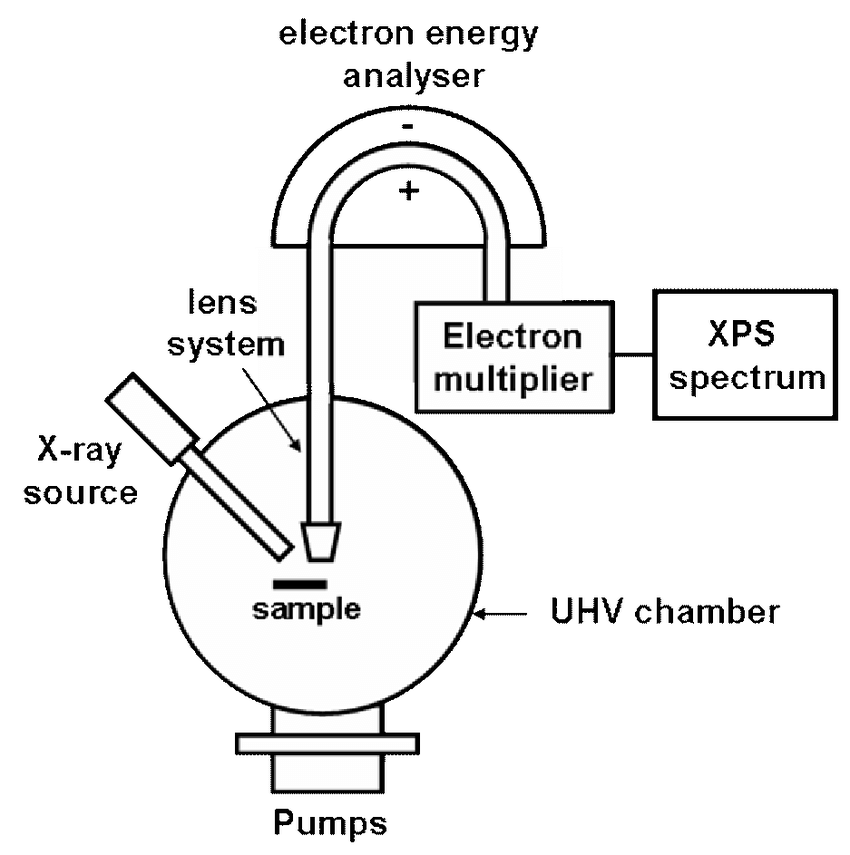
\includegraphics[width=0.75\textwidth]{Chapter2/Figs/2f.png}
\caption[Schematic representation of an XPS system.]{Schematic of an XPS instrument. The X-ray radiation interacts with the sample and emitted electrons are focused onto the analyser which measures their kinetic energies and indirectly their binding energies \cite{regonini2008anodised}. }
\label{fig:2f}
\end{figure}

\noindent Figure \ref{fig:2f} depicts a schematic representation of an XPS system. An X-ray source is employed to irradiate the sample, which is situated within a vacuum chamber. A vacuum pump is connected to the system, enabling the reduction of the pressure to a range of $10^{-8}$ to $10^{-9} mbar$ for the purposes of analysis. The ejected photoelectrons are detected by means of electronic lenses. It is possible to adjust the voltages during this process in order to select electrons of a specific kinetic energy. \\

\noindent A hemispherical analyser (HSA), which comprises a pair of charged plates, is employed to select electrons of specific energy (also referred to as 'pass energy'). The electron detector quantifies the flux of incoming photoelectrons with the specified pass energy, a process also designated as 'fixed analyser transmission' (FAT) mode. By varying the lens voltage across a range of electron energies to ascertain the variation in flux at the detector, the spectrum of the measured sample can be generated and displayed.\\


\noindent In order for the incident radiation to ionise matter and extract its electrons, the energy of the radiation must be sufficient to eject electrons into the vacuum. The energy required for this process is known as the binding energy $E_{b}$ for core electrons. The electron energy $E_k$ can be expressed in terms of the incident x-ray energy $h\upsilon$, where $h$ is Planck's constant and $\upsilon$ is the photon frequency, the sample work function $\phi$, and the electron binding energy , as follows:
\begin{align}
E_k = h\upsilon - E_{b} - \phi \label{eq:2.20}
\end{align}

\noindent In a given spectroscopic measurement, the frequency $\upsilon$ is known and the constant of Planck's law of radiation, $h$, is constant. Consequently, the energy of electrons in the conduction band, $E_b$, can be measured to estimate the energy of electrons in the valence band, $E_k$. The latter varies depending on the element, and therefore different peaks characterising the composition of the sample will appear in the XPS spectrum.\\

\noindent X-ray radiation has the capacity to penetrate deeply into a sample, yet only electrons situated in close proximity to the surface are able to escape. As a consequence of the high degree of scattering that occurs within the sample, the photoelectrons generated are subject to a significant loss of energy. The surface sensitivity of the technique is determined by the low escape depth (0.5-2 nm) of the elastically scattered electrons \cite{oswald2006x}.\\

\noindent The energy resolution of the measured spectrum is susceptible to a number of parameters. These parameters include the diameter of the analyser, the energy spread of the X-ray source, and the pass energy. Conversely, the ionisation process results in the formation of localised charges at the surface of the sample (sample charging). \\

\noindent The presence of these localised charges may result in a broadening of the spectrum lines. It is therefore necessary to implement an effective charge neutralisation process. This is achieved by injecting electrons into the vacuum chamber using an ion gun, which neutralises the tested sample and improves its photoelectron emission. \\

\noindent It should be noted that the pass energy of the detector determines the energy of the electrons that are detected, and thus the detector energy resolution. This quantifies the ability to resolve peaks that differ in energy by a small amount. The lower the energy pass, the greater the resolution power of the analyser.\\

\noindent In contrast, Auger peaks manifest at elevated binding energies. Radiation-induced photoemission gives rise to shell vacancies, which can be filled by excited electrons undergoing decay and emitting Auger electrons. X-ray emission can also occur during the ionisation process in heavy atoms. Many samples exhibit degradation under exposure to X-rays.\\

\noindent The probing method frequently permits focusing the X-ray beam onto a narrow, specific spot, thereby reducing sample damage to an absolute minimum. Despite XPS being a surface analysis technique, depth profile measurement can be performed nonetheless \cite{geng2002xps}. This can be typically achieved by integrating an ion beam source into the XPS system to mill the sample. \\

\noindent Through ion milling, the sample material can be removed in a sequential manner while its composition is characterised. However, the milling process may result in alterations to the composition and cause damage to the sample. The introduction of energetic ions during the milling process may also result in the implementation of material, leading to changes in the composition with depth.


\subsection[Model Fitting Framework]{Model Fitting Framework}

This section presents the development of empirical models designed to track the rates of increase and decrease in conductance separately. The models are primarily intended to quantify the rate of change in conductance. The question of a physical model will be addressed in the following section.\\

\noindent The models explored here are derived from the relaxation experiments that were previously outlined in the preceding chapter. It was evident that the gradual decline in device current delineated the upper limit of the maximum device current, while the initial surge in current approached this maximum but did not exceed it. 
\begin{align}
I(t) = f_{inc}(t) \times f_{dec}(t) \quad \forall \left\{ f_{inc}(t) \in [0 \to 1] : f_{dec}(t) \in \mathbb{R} \right\} \label{eq:2.21}
\end{align}

\noindent This is represented by the product of two time-dependent functions, $f_{inc}(t)$ and $f_{dec}(t)$. The increase in current is analogous to a charging term, $f_{inc}(t)$, which rises from 0 to 1. Initially, this function defines the device current. However, as $f_{inc}(t)$ approaches 1, it then allows the function it is multiplied with to define the total current, in this case  $f_{dec}(t)$. \\

\noindent Although this equation forms the basis of the empirical model, questions remain regarding the specific forms that $f_{inc}(t)$ and $f_{dec}(t)$ should take and the most appropriate means of comparing their effectiveness. The efficacy of each fitting equation is evaluated based on two criteria: the quality of the fit and the degree of realism of the fitted parameters in relation to the underlying physical system from which the model is derived.\\

\noindent The correspondence between each term of a given model and a physical property is contingent upon the physical system from which the model is derived. These properties are assigned a range of values that are deemed realistic. Values outside of this range may indicate that the assumed model is not applicable. The specific correspondence between physical properties and terms is model-specific and will be detailed later in conjunction with the model.\\

\noindent The discrepancy between the fitted equation and the original experimental data is referred to as the residual. This can often be a useful visual indicator of the quality of the fit. An optimal fit would manifest residuals that are centered around zero, exhibiting no systematic offsets or time-variant components. \\

\noindent The residuals in this form indicate that the fitted equation tracks the experimental data well, with the variances in the residuals around zero assumed to be a form of noise or variance in the original data. In contrast, a less optimal fit would exhibit systematic offsets that vary over time. This indicates that either an additional term is absent or the incorrect function has been selected. \\

\noindent However, while residuals are useful for visually assessing a fit, they are less so when larger datasets are being fitted. Therefore, only one residual for each model is assessed, which is representative of the model's performance. The same experimental data will be fitted for each model, thus ensuring an accurate comparison. In order to assess a model's goodness of fit across a whole dataset, a single numerical metric that can quantify the fit is preferred.\\

\noindent A more quantitative description of the goodness of fit is provided by the $R^2$ measure. The $R^2$ measure is a statistical tool that enables the comparison of the variance between the observed data points and the model's predicted values against the variance of the observed data and the mean of that data. In other words, it can be acknowledged that the most straightforward model for predicting a dataset would be to assume the mean value of the dataset in all cases.
\begin{align}
SS_{tot} &= \sum_{i}\left( y_i - \bar y \right)^2 \label{eq:2.22} \\
SS_{res} &= \sum_{i}\left( y_i - f_i \right)^2 \label{eq:2.23} \\
 R^2 &= 1 - \frac{SS_{res}}{SS_{tot}} \label{eq:2.24} 
\end{align}

\noindent In this case, the variance is defined by (\ref{eq:2.22}), Where $y_i$ is an individual datapoint and $\bar y$ is the mean average of the dataset, which is equal to the variance of the dataset. The variance of the dataset against the model's predictions can also be calculated with (\ref{eq:2.23}), Where $f_i$ is model’s predicted value at $i^th$ index, for any other model developed. \\

\noindent If the variance is similar to that of the dataset, the model is no more than a simple mean value predictor, and thus the data fit is poor. An alternative indication of a good fit is provided by a model with a variance much less than that of the dataset. However, residuals should still be checked. The $R^2$ value shown in (\ref{eq:2.24}), defined by the ratio of the variance of the model to the variance of the dataset, is based on this premise and increases as the model's fit improves.\\

\noindent Notwithstanding the possibility of attaining an optimal fit, the values of the fitted parameters remain uncertain. To illustrate, a minimum in the fitting error could be achieved by a range of parameter values. This range is referred to as the confidence bounds, which can be interpreted as the range within which the fitting algorithm is certain the final value lies. \\

\noindent For example, 90\% confidence bounds will define a range within which the algorithm is 90\% sure the optimal value can be found. If a higher confidence is required, the range will generally increase. Consequently, there is a trade-off between certainty and specificity. In this work, the standard confidence threshold of 90\% was employed.\\

\noindent The choice of model for a particular dataset is influenced by the magnitude of the confidence intervals. If a model results in fitted parameters with large confidence intervals, it can present a challenge when interpreting the results, particularly if the changes in these values are small. Consequently, when selecting a model for the analysis of a dataset, preference will be given to models with smaller intervals.

\subsection[Empirical Model Definition]{Empirical Model Definition}

The current transients observed in amorphous silicon oxide devices appear to result from two distinct changes occurring within the device simultaneously, leading to both an increase and a decrease in conductance. The two changes in conductance exhibit a number of distinguishing characteristics. \\

\noindent Firstly, the increase in conductance occurs significantly faster than the subsequent decay. Secondly, in terms of volatility, the increase in conductance relaxes to its initial state within tens of milliseconds, whereas the decay in conductance can take hours to fully reset. Thirdly, in terms of their material dependence, the decay in conductance can be removed by changing the material of the electrodes \cite{mannion2022current}. \\

\noindent This has led to the conclusion that the two changes are driven by different mechanisms and can exist in isolation, which will be detailed in the following sections. The SPICE models for each of these processes will first be presented separately, and then the two will be combined to obtain the final model.

\begin{figure}[htbp!] 
\centering    
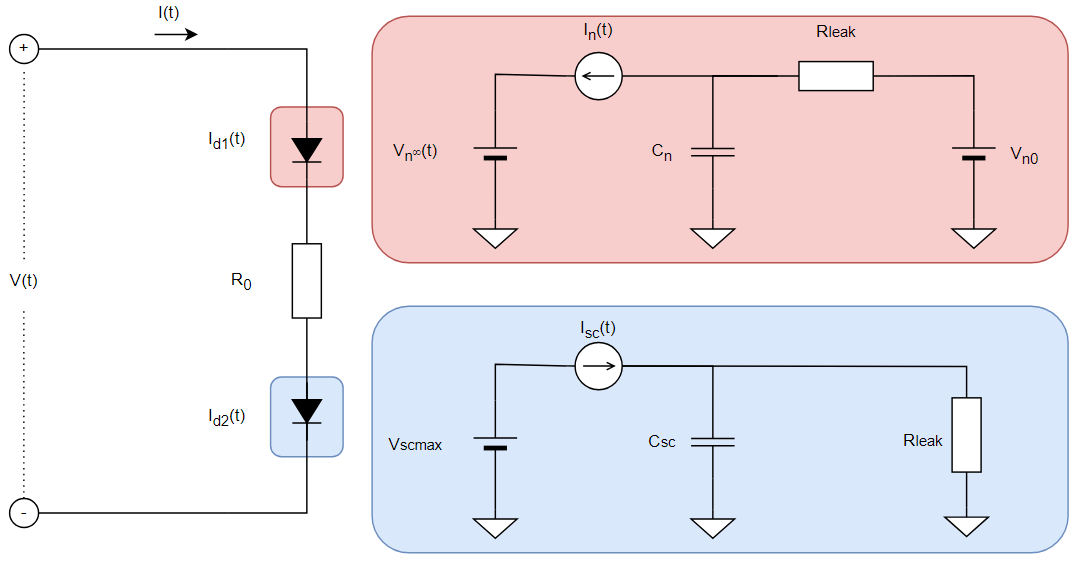
\includegraphics[width=1\textwidth]{Chapter2/Figs/2g.png}
\caption[SPICE Model diagram.]{SPICE Model diagram. The SPICE model generates an output current, \textit{I(t)}, based on an input voltage, \textit{V(t)}. The circuit incorporates a single resistor, $R_0$, along with two diode models that serve to attenuate or amplify the voltage applied to the resistor. These diode models are represented by the sub-circuits highlighted in blue and red.}
\label{fig:2g}
\end{figure}

\noindent The accelerated rise in conduction appears to be attributable to the phenomenon of charge trapping. This is corroborated by its shorter timescales, greater volatility, and experiments in which optically injected carriers were demonstrated to accelerate the process. One potential mechanism by which charge trapping affects device conductance is through modulation of the height of a Schottky-like barrier \cite{cowley1965surface}, which may be influenced by the population of interface states \cite{sze2021physics}. \\

\noindent Although Schottky barriers are typically formed between metal-semiconductor interfaces, studies have identified analogous barriers within memristor devices \cite{hansen2015double}. The silicon oxide devices exhibit rectifying behaviour, indicating the presence of an interface barrier at one of the metal-insulator interfaces. Additionally, the filaments in the devices are composed of silicon-rich regions within the oxide, suggesting that the interface between these filaments and metal contacts may resemble a Schottky interface.\\

\noindent The Schottky barrier is modelled as a voltage drop, which acts to reduce the voltage across the active layer of the device, as illustrated in \ref{fig:2g}. As the height of the Schottky barrier diminishes, the potential across the active layer increases, resulting in a greater device current. The voltage drop resulting from the Schottky-like barrier is a function of time and is modelled using the sub-circuit illustrated in red in \ref{fig:2g}. \\

\noindent The magnitude of the voltage drop is represented within the sub-circuit by the voltage across the capacitor, $C_n$. The initial value of the aforementioned variable is discharged by the current source, $V_{n0}$. The rate of discharge is defined by the current source, $I_n(t)$, whose magnitude is proportional to the difference between the current voltage drop across the Schottky barrier and its final equilibrium value, $V_{n\infty}$.
\begin{align}
I_n(t) = \alpha \times \left[ V_n(t) - V_{n\infty} \right] \label{eq:2.25} 
\end{align}

\noindent In this equation, $\alpha$ corresponds to the probability of trapping a carrier, while the voltage difference relates to the concentration of unpopulated states. The current source discharges the capacitor to a final equilibrium voltage, $V_{n\infty}$, where the trapping and de-trapping currents are equal. An additional leaking resistor, $R_{leak}$, is introduced to correctly adjust for the rectifying behaviour of the device.\\

\noindent There is compelling evidence that the observed decline in conductance can be attributed to the movement of charged ions within the oxide thin film. This hypothesis has been put forth in the majority of publications on such current transients \cite{wang2006oxygen}. This is largely based on the observation that the decay in conductance occurs over a time scale of tens to hundreds of seconds, which is too long to be associated with the trapping of electrons or holes. \\

\noindent Furthermore, in accordance with the drifting defect hypothesis, it has been demonstrated that the process can be reversed by applying a voltage of opposite polarity, despite the device exhibiting significantly reduced currents in the opposite polarity. The model adhere to this approach and hypothesise the presence of migrating defects. Of particular significance is the assumption that the ionic current induced by the migrating space charge is negligible in comparison to the electronic currents, as predicted \cite{meyer2005oxygen}. \\

\noindent It is assumed that the electronic current flows through a conductive channel within the oxide. In our silicon oxide devices, this is a silicon-rich filament that forms during electrical stressing. Such filaments are common in memristors and have been observed in our devices using etching C-AFM techniques \cite{buckwell2015conductance}.\\

\noindent In order for an electronic current to be induced through these filaments, it is necessary that a potential be present across the channel. In our model, the migrating space charge modulates the current by reducing the potential experienced along the filament. It is probable that this space charge is a positively charged ion that has accumulated in proximity to the upper gold electrical contact. This assertion is corroborated by the observation that the impact of the accumulation of space charge can be negated by modifying the material of the top electrical contact from gold to indium tin oxide \cite{mannion2022current}.\\

\noindent The precise nature of this ion remains uncertain. A substantial amount of oxygen migration and associated oxygen vacancies have been observed throughout the device when under bias \cite{vanka2022hydrogen}, indicating that this could be a viable candidate. However, in other devices, hydrogen has been identified as a defining factor in device behaviour. Additionally, hydrogen has been detected in significant quantities within our devices \cite{lagarias1998convergence}. Given the lack of certainty regarding the identity of the ion, we assume a generic space charge.\\

\noindent The effect of the space charge on the conductive channel can be described as follows. In the initial phase, the space charge exhibits a homogeneous distribution. Upon the application of a voltage to the device, a force is imparted on the space charge, resulting in its drift and accumulation at the device electrode. This accumulation effectively blocks the space charge from exiting the oxide.  \\

\noindent This accumulation results in the formation of a region of higher space charge concentration, which consumes a portion of the potential applied across the device. This results in a reduction in the potential drop across the conductive channel. As the space charge accumulates, this voltage drop increases, meaning less potential is dropped across the channel and a reduction in device current is observed. \\

\noindent Eventually, the drifting force imparted on the space charge will reach equilibrium with the diffusion and Coulombic repulsion formed by the accumulated space charge, leading to a steady state condition. When the potential is removed, the space charge diffuses back to its original distribution. \\

\noindent The aforementioned process is modelled using the circuit illustrated in Figure \ref{fig:2g}. The conductive channel is represented by a fixed resistance, designated as $R_0$. The voltage across the conductive channel is defined by the applied potential at the terminals of the device, $V(t)$, and the voltage source, $V_{sc}(t)$, which represents the voltage drop caused by the accumulated space charge. This voltage source is time-dependent and is defined by the subcircuit shown in blue. As the voltage of this source increases over time, the voltage across the fixed resistor drops and the device current also reduces.
\begin{align}
I_{sc}(t) = \left[ V_{scmax} - V_{sc}(t) \right] \times \left[ \mu \left( V(t) - V_{sc}(t) \right) \right] \label{eq:2.26} 
\end{align}

\noindent The blue sub-circuit illustrated in \ref{fig:2g} is responsible for monitoring the accumulation of the space charge and its corresponding voltage drop, which is represented by the voltage across the capacitor $C_{sc}$. The capacitor is charged by the current source, $I_{sc}(t)$, which generates a current in (\ref{eq:2.26}). The capacitor is defined by the voltage applied across the device and $\mu$, which symbolises the mobility of the space charge. The current source draws charge from a voltage source representing the steady-state voltage drop, i.e. the maximum voltage drop consumed by the accumulated space charge $V_{scmax}$.
\begin{align}
I_d(t) = \left( I_0 + I_{\delta} V_n(t) \right)\times \left( e^{\frac{V(d_1,d_2)}{nV_t} }  - 1\right) \label{eq:2.27}
\end{align}

\noindent To complete the model, the subcircuits for both potential drops are combined as illustrated (\ref{eq:2.27}). The two voltage drops act upon a single resistor representing the conductive channel, $R_0$. In practice, this channel does not exhibit ohmic conduction and thus its resistance will have a voltage dependence. This is taken into account while collecting the meta-parameters.

\section[Results]{Results}

\subsection[Conductance Variation Mechanisms]{Conductance Variation Mechanisms}

The initial step is to ascertain the location within the device stack where alterations are taking place that are responsible for the observed reduction in conductance. The absence of decay occurring concurrently with the alteration of the top electrode suggests that the causal factor responsible for the observed conductance decay is situated at the interface between the top electrode and the amorphous silicon dioxide. \\

\noindent Given the slow dynamics of the change in conductance, it is plausible that a drift of some mobile defect is responsible. It is well established that silicon dioxide films are susceptible to the influence of alkali mobile ions \cite{snow1965ion}, including sodium and lithium ions, which are all characterised by a positive charge \cite{yon1966sodium}. The drift of these mobile charges can significantly affect the potential drops at metal-oxide interfaces, as well as modulate barrier heights when allowed to accumulate.\\

\noindent If some positive mobile ion, regardless of the species, existed in the oxide of the device, it would be attracted to the top electrode, which is at a negative potential. This would cause an accumulation of positive space charge at the interface, which would in turn reduce the potential across the oxide. Nevertheless, it can be argued that alkali metals, such as sodium and potassium, are unlikely to be the cause of this positive space charge, given that they do not migrate at room temperature. \\

\noindent Instead, they require temperatures in excess of 100 degrees Celsius (212 degrees Fahrenheit) \cite{deal1974current}. The current transients presented in this thesis are all observed at room temperature, which suggests the need for an alternative candidate to explain the mobile space charge, in particular one that is mobile at room temperature. \\

\noindent It is noteworthy that modelling of the temperature within analogous $TaO_x$ devices has indicated the potential for increases in oxide temperature of up to 100°C with applied voltages of -0.7 to -1.8V due to Joule heating \cite{shen2021experimentally}. This would imply that if comparable effects were present during the current transient, then elevated temperatures within the oxide could be occurring and potentially facilitating the migration of alkali metal defects.\\

\noindent It seems plausible to suggest that the proton \cite{hofstein1967proton} is a likely candidate for positive ions that are mobile at room temperature. The presence of ionised hydrogen in silicon dioxide films has been repeatedly observed to be both stable and consistent \cite{vanheusden1998chemical}. It has been demonstrated that protons can influence the electronic properties of capacitor devices in which protons are trapped within the oxide \cite{vanheusden1999non}. Their long-term stability has been demonstrated through multiple cycles of migration between device electrodes \cite{warren1997protonic}. \\

\noindent It is commonly assumed that these ions are introduced during the growth of the oxide \cite{vanheusden1998thermally}. Furthermore, their concentration has been demonstrated to increase through annealing in an atmosphere at temperatures above 200 degrees Celsius \cite{lifshitz1989detection}. However, their presence has also been introduced electronically via the electrolysis of water within the device and via radiation \cite{winokur1977field}. It is also noteworthy that their migration has been shown to occur repeatedly at room temperature.\\

\noindent This raises the question of why the accumulation of protons occurs exclusively in the gold-contacted devices, rather than in the ITO. Given that gold is an inert metal and is unlikely to be reduced by protons, the accumulation at the gold interface is to be expected. In contrast, there is a substantial body of evidence indicating that the ITO would be reduced in the presence of protons.\\

\noindent Although ITO contacts are often considered to be inert in certain electrochemistry scenarios, this is not always the case. Their reduction is, in fact, heavily dependent on the pH of the electrolyte. For instance, the reduction of the electrode has been observed on numerous occasions in acidic electrolytes \cite{ciocci2021differentiating,senthilkumar2008electrochemical}. \\

\noindent The reduction of ITO in the presence of acids has been demonstrated in both electrochemical experiments conducted at room temperature \cite{wang2003optical} and in instances where ITO has been exposed to a hydrogen plasma \cite{banerjee1987degradation}. In one study, the application of negative voltages to an ITO electrode immersed in hydrochloric acid resulted in the formation of spherical structures at the grain boundaries of the ITO film, which exhibited a metallic-like appearance [88]. \\

\noindent Following characterisation with Energy dispersive x-ray Spectroscopy (EDS) \cite{huang2003electrochemical} and X-ray Diffraction (XRD) in a separate study \cite{liu2015important}, the spherical regions were found to be depleted of oxygen or exhibited only peaks of indium and tin, providing compelling evidence that these spheres were metallic. The same spherical structures were observed in ITO films exposed to a hydrogen plasma, which, when analysed with Auger spectroscopy, again revealed a lower oxygen concentration in the spherical regions.\\

\noindent The reduction of ITO by protons may provide an explanation for the absence of space charge accumulation in ITO-contacted devices. Instead of accumulating, the protons reduce the ITO, producing water as a byproduct, which would not contribute to a positive space charge. Furthermore, the reduction of the electrode may also elucidate the more erratic current-time response observed in ITO devices, as the electrode structure undergoes substantial alterations.\\

\noindent The potential for structural changes to occur in both the oxide and the metal contacts makes it challenging to determine the specific role each plays in modulating the device's conductance. In order to investigate the effect of the contact, it would be beneficial to fabricate and characterise devices with a variety of contact materials. \\

\noindent Any discrepancies in the observed behaviour between the devices could be ascribed to the metal or the metal-insulator interface, whereas any enduring effects could be attributed to the oxide. To further examine any behaviour attributed to the oxide, devices of varying oxide thicknesses could be fabricated. This may reveal a dependence on the oxide thickness, which could be supporting evidence for the oxide having a role in the changing device conductance. \\

\noindent However, it is important to exercise caution when drawing conclusions from this approach, as the change in oxide thickness will also modify the magnitude of the current density flowing through the device, potentially affecting the interfaces. The fabrication of devices with different oxide thicknesses and a variety of metal contacts is a future research direction. \\

\noindent If the hypothesis that the transient is the result of two separate changes is true, then it would suggest that devices could potentially be made to exhibit only one of these changes in isolation. Fabrication of such a device would provide strong supporting evidence for the hypothesis and a clear demonstration that the changes are separable. Modification of the top contact material appears to facilitate this separation.\\

\begin{figure}[htbp!] 
\centering    
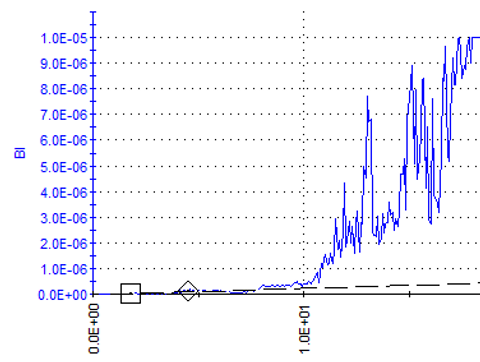
\includegraphics[width=0.5\textwidth]{Chapter2/Figs/2h.png}
\caption[The current-time response for a device with a conductive ITO top electrode.]{The current-time response for a device with a conductive ITO top electrode. The current is generated in response to a step potential applied to the top contact with respect to the bottom. It exhibits only the increase in conductance and not the decrease. As the current increases, the noise level also rises until the device reaches a point of breakdown. The structure of the device is identical to that of the gold-contacted devices, with the exception of the change in the top electrode's material from gold-titanium to indium tin oxide (ITO).}
\label{fig:2h}
\end{figure}

\noindent Devices fabricated with a conductive ITO top electrode, in lieu of the gold-titanium contact, do not exhibit the anticipated decay in conductance; rather, they display only the initial increase. Figure \ref{fig:2h} illustrates the current-time response of an ITO-contacted device. As observed previously in the gold devices, the current begins to increase; however, it never reaches the inflection point. Instead, it continues to increase in conductance, becoming progressively noisier until the device undergoes breakdown.\\

\noindent The ITO device has undergone a comparable stressing process to that of the gold devices, which is outlined in the preceding chapter. In the initial stages, the devices exhibit only capacitive currents and possess a very high resistance. Subsequently, a constant current stressing procedure is employed to produce a more conductive device. \\

\noindent Following a period of relaxation, a repeatable transient is produced, provided that the applied voltage is maintained for a sufficiently brief duration to prevent breakdown of the device. A comparable phenomenon has been documented \cite{moon2019rram} in a variety of oxides and is frequently employed in the replication of short-term potentiation of synapses \cite{zhang2017emulating, chang2011short}.\\

\noindent Furthermore, this absence of slower dynamics may corroborate with previous findings \cite{meyer2005oxygen}, where the slower dynamics were postulated to be attributable to oxygen vacancies. It is conceivable that the ITO contact is more prone to exchange oxygen with the oxygen vacancy than the inert gold contact. \\

\noindent An alternative hypothesis is that the Au contact is diffusing through the oxide, whereas the ITO contact is not. Previous observations have shown that Au can form conductive bridges between two contacts through a thin film of $ZnO$ \cite{peng2012resistive}. Given that gold is known to diffuse in silicon dioxide films, this could be a possibility \cite{madams1974migration}. However, TEM analyses of the devices studied in this thesis have not produced observable gold filaments, casting doubt on this hypothesis \cite{mehonic2017intrinsic}.\\

\noindent An additional potential explanation for the observed discrepancy in behaviour between the Au and ITO contacts is the possibility of differences in their respective work functions. While not directly measured on the samples in question, the work function of gold is reported to be between 4.9 and 5.2 electronvolts (eV) \cite{tran2019anisotropic}, while thin films of indium tin oxide (ITO) have been measured to have a work function between 4.25 and 4.28 eV \cite{schlaf2001work}. \\

\noindent This could result in a difference in work function of approximately 1 eV. Such differences would lead to offsets in the band alignments at the contact and oxide, which could affect which traps within the oxide the electrons are injected into. As discussed in the previous chapter, the disappearance of the slower decay in conductance with the change in top electrode is suggestive of proton migration playing a role in the slower decay in device current.

\subsection[Oxygen Exchange Experimentation]{Oxygen Exchange Experimentation}

\subsection[Model Fitting and Evaluations]{Model Fitting and Evaluations}


\section[Conclusion]{Conclusion}


\noindent Neuromorphic modelling is therefore concerned with the creation of artificial systems that emulate the functionality of biological neural systems, particularly in terms of their physical implementation. The term was first used in the late 1980s to describe digital and analogue hardware that is organised in a more brain-like manner than traditional computer hardware \cite{mead1990neuromorphic}. \\

\noindent One of the fundamental concepts underlying neuromorphic systems is parallel distributed processing. Neuromorphic systems arrange computations at the neural level, with a specific focus on facilitating rapid communication between neural processing units. This contrasts with other parallel distributed systems, such as graphics processing units (GPUs), which are typically optimized for independent parallel computations and exhibit limited communication between units.